\documentclass[pdflatex,sn-mathphys-num]{sn-jnl}

\usepackage{amsmath,amssymb,amsfonts,bm}
\usepackage{booktabs}
\usepackage{multirow}
\usepackage{makecell}
\usepackage{tabularx}
\usepackage{array}
\usepackage{graphicx}
\usepackage{xcolor}
\usepackage{algorithm}
\usepackage{algorithmic}
\usepackage{enumitem}
\usepackage{float}
\providecommand{\FloatBarrier}{\relax}
\usepackage{url}
\usepackage{hyperref}

%% Relaxed Float Placement Parameters (Prevents Float Drift / Queue Congestion)
\renewcommand{\topfraction}{0.95}
\renewcommand{\bottomfraction}{0.85}
\renewcommand{\textfraction}{0.05}
\renewcommand{\floatpagefraction}{0.80}
\setcounter{topnumber}{5}
\setcounter{bottomnumber}{4}
\setcounter{totalnumber}{8}

%% Theorem Environments (using sn-jnl predefined styles)
\theoremstyle{thmstyleone}
\newtheorem{theorem}{Theorem}
\newtheorem{lemma}{Lemma}
\newtheorem{proposition}{Proposition}
\newtheorem{corollary}{Corollary}

\theoremstyle{thmstylethree}
\newtheorem{definition}{Definition}
\newtheorem{remark}{Remark}


%% Math Operators and Notations
\DeclareMathOperator*{\argmax}{arg\,max}
\DeclareMathOperator*{\argmin}{arg\,min}
\DeclareMathOperator{\Simplex}{Simplex}
\DeclareMathOperator{\EMA}{EMA}
\DeclareMathOperator{\ReLU}{ReLU}
\DeclareMathOperator{\Cosine}{Cos}
\DeclareMathOperator{\clip}{clip}

%% Metric and Symbol Macros
\newcommand{\MethodName}{FU-Alignment}
\newcommand{\MethodVariantFull}{FU-Alignment (full)}
\newcommand{\dpd}{\mathrm{DPD}}
\newcommand{\dpdhard}{\mathrm{DPD}_{\mathrm{hard}}}
\newcommand{\eod}{\mathrm{EOD}}
\newcommand{\wadv}{w_{\mathrm{adv}}}
\newcommand{\OmegaW}{\Omega_w}
\newcommand{\Rstar}{\mathcal{R}^*}
\newcommand{\Droot}{D_{\mathrm{root}}}
\newcommand{\gtarg}{g_{\mathrm{target}}}
\newcommand{\gtask}{g_{\mathrm{task}}}
\newcommand{\gfair}{g_{\mathrm{fair}}}
\newcommand{\ip}[2]{\langle #1, #2 \rangle}
\newcommand{\norm}[1]{\left\lVert #1 \right\rVert}
\newcommand{\EE}{\mathbb{E}}
\newcommand{\RR}{\mathbb{R}}

% Allow extra inter-word stretch before a line overflows the margin
\setlength{\emergencystretch}{2em}

\newcommand{\codeurl}{\url{https://github.com/ngngsonan/TrustFedGNN}}

\begin{document}

\title[TrustFedGNN]{TrustFedGNN: Auditing and Mitigating Report-Dependent Trust in Federated Graph Learning}

\author[1]{\fnm{Ngoc-Son-An} \sur{Nguyen}}

\author*[2]{\fnm{Quang-Vinh} \sur{Dang}}

\author[1]{\fnm{Tuong-Nguyen} \sur{Huynh}}

\affil[1]{\orgname{Industrial University of Ho Chi Minh City}, \orgaddress{\city{Ho Chi Minh City}, \country{Vietnam}}}

\affil*[2]{\orgname{British University Vietnam}, \orgaddress{\city{Hung Yen}, \country{Vietnam}}}

\abstract{Lenders and public agencies increasingly train graph neural networks jointly without pooling data. To keep such federations fair, several aggregation rules weight each client by the loss or disparity it reports about itself, which the server cannot verify. We audit this interface with a fixed-update intervention that changes only an adversary's report while client updates and server state stay constant. Across 30 seeds, all six report-dependent rules shift weight towards the adversary, by up to 0.91, whereas rules that read no report keep identical aggregates. We then propose TrustFedGNN, whose server rule, FU-Alignment, ignores client reports. It clips each update, scores it by projection onto a reference gradient from a small confidential server graph, and smooths the signed score over rounds. Under matched fairness poisoning, FU-Alignment lowers the adversary's mean weight relative to root-update FLTrust from 0.189 to 0.063 on German Credit and from 0.196 to 0.045 on Bail, with higher AUC on both datasets. An ablation attributes this gain to clipping and signed smoothing. Under adaptive reference evasion, FU-Alignment gives attackers the lowest weight and influence of four rules and retains the highest AUC; attackers that alternate honest and poisoning phases on German mark its boundary. On Pokec-z, its AUC is non-inferior to FedAvg's at a prespecified 0.01 margin. The study thus offers a reusable audit and an inspectable, report-independent aggregation rule with a mapped operating boundary.}

\keywords{Federated Learning, Graph Neural Networks, Byzantine Robustness, Algorithmic Fairness, Trust Auditing}

{\renewcommand{\thefootnote}{}\footnotetext{\hspace*{-1.8em}\textbf{*}Corresponding author: Quang-Vinh Dang (\href{mailto:vinh.dq4@buv.edu.vn}{vinh.dq4@buv.edu.vn}). Contributing authors: Ngoc-Son-An Nguyen (\href{mailto:annns25871@pgr.iuh.edu.vn}{annns25871@pgr.iuh.edu.vn}); Tuong-Nguyen Huynh (\href{mailto:huynhtuongnguyen@iuh.edu.vn}{huynhtuongnguyen@iuh.edu.vn}).}}
\maketitle

%% =========================================================================
%% MODULAR MANUSCRIPT SECTIONS
%% =========================================================================

\section{Introduction}
\label{sec:introduction}

Federated graph learning lets institutions train graph neural networks without pooling their subgraphs~\citep{kipf2016semi,velickovic2017graph,mcmahan2017communication,kairouz2021advances}. In credit and risk applications, however, collaboration must address both group disparities and malicious participants. Several fairness-aware aggregation rules weight clients using locally reported losses or fairness statistics~\citep{ezzeldin2023fairfed,li2020fair,f2gnn2023,khan2026fedgraphfair,bendoukha2025popets,dang2026fedfairgnn}. Those statistics may be useful under honest participation, but the server cannot usually verify them without access to private client data. Consider a consortium of lenders that trains a credit-risk model on its members' customer graphs. If one member can raise its own aggregation weight by reporting a small disparity and a low loss, it can steer the shared model while appearing to be the most responsible participant, and no other member can detect this from the reports alone.

This paper asks a concrete operational question: what happens when an aggregation rule treats a self-reported scalar as evidence of client quality? We first separate that interface dependency from training dynamics. In a fixed-update intervention, client updates and server state remain identical while the adversary changes only its report. The resulting weight change measures the direct sensitivity of the rule to unverified telemetry. The audit identifies a manipulable input and measures how much weight each rule concedes through it; rules that read no report act as controls whose invariance confirms that the intervention isolates the report channel.

We then introduce TrustFedGNN and its server rule, FU-Alignment. The server holds a small confidential audit graph, computes task and fairness reference gradients on it, clips client updates, and weights them by signed, temporally smoothed projections onto the combined reference. The aggregation path consumes no client-reported loss or disparity. Server anchoring itself is established by FLTrust~\citep{cao2021fltrust}; our contribution is the score dynamics (clipping before projection scoring and signed smoothing before rectification), whose effect we isolate by ablation, and an audit design that tests report dependence and adaptive-access boundaries.

The evidence supports three conclusions:
\begin{enumerate}[leftmargin=*]
    \item \textbf{Report-surface audit.} In a fixed-update audit, changing only the adversary's report changes its mean weight under six report-dependent rules, while CGSV, FLTrust, root-update FLTrust, and FU-Alignment produce bit-identical aggregates under a report falsified in every field except the sample count. An end-to-end run confirms the invariance for root-update FLTrust.
    \item \textbf{Controlled mechanism evidence.} Under a controlled fairness-poisoning protocol, FU-Alignment assigns less adversarial weight than root-update FLTrust on German (0.0630 versus 0.1892) and Bail (0.0451 versus 0.1959), with higher AUC on both datasets in the same matched runs. A factorial ablation attributes the reduction to clipping and signed smoothing; the fairness term has no detectable effect at the weight used.
    \item \textbf{Explicit boundaries.} An adaptive-access study shows that performance depends on dataset and adversarial access: under reference evasion FU-Alignment gives the adversaries the lowest weight and influence of the four rules compared and keeps the highest AUC on both datasets, and on Bail it has the lowest processed influence under sustained and intermittent poisoning; Section~\ref{subsec:rq4_boundary} identifies the access pattern under which this advantage does not hold. A known-label control supports AUC non-inferiority to FedAvg on Pokec-z observed labels, but does not support fairness superiority.
\end{enumerate}

\paragraph{Relation to prior work}
FSER and FTGD adapt ideas from our earlier FedFairGNN study~\citep{dang2026fedfairgnn} and are held fixed across relevant comparisons. They are not contributions of this paper. The present contribution lies in the trust-surface audit, the FU-Alignment server rule, and the evidence-backed characterization of its operating boundary.

Section~\ref{sec:related_work} positions the work against fairness-aware aggregation and server-anchored trust. Section~\ref{sec:methodology} defines the threat model and method. Section~\ref{sec:experiments} presents the evaluation, Section~\ref{sec:discussion} discusses deployment and limitations, and Section~\ref{sec:conclusion} summarizes the supported conclusions.

%% sections/02_related_work.tex
\section{Related Work and Setting}
\label{sec:related_work}

We review fairness-aware federated graph learning (Section~\ref{subsec:rw_fairfl}), privacy limitations of reported fairness statistics (Section~\ref{subsec:rw_privacy}), Byzantine-robust aggregation and server-anchored trust (Section~\ref{subsec:rw_robust}), client contribution evaluation (Section~\ref{subsec:rw_contribution}), and the architectural relation to prior work (Section~\ref{subsec:rw_prior_work}).

\subsection{Fairness in Federated Graph Learning}
\label{subsec:rw_fairfl}

Graph neural networks~\citep{kipf2016semi, velickovic2017graph} trained under federated protocols~\citep{mcmahan2017communication, kairouz2021advances} enable collaborative inference over distributed subgraphs without pooling raw adjacency or feature matrices. Two principal paradigms address group fairness in this setting.

The first paradigm operates within client-side local training while leaving the global aggregation mechanism unmodified. FairGNN~\citep{dai2021say} employs adversarial training to purge sensitive demographic attributes from node representations, and FairSIN~\citep{yang2024fairsin} neutralizes sensitive signals in feature space. Related methods rebalance graph topologies~\citep{li2024fairgb}, learn invariant representations~\citep{zhu2024fairinv}, debias input structures~\citep{dong2022edits}, optimize fair contrastive objectives~\citep{agarwal2021towards}, or disentangle sensitive latent factors~\citep{lee2025dabgnn, fnrgnn2025}. In vertical federations, FAVGNN~\citep{wang2026favgnn} addresses feature-split graphs. Because client-side debiasing mechanisms execute locally, they provide no systemic defense if a participating client deliberately manipulates its training objective or falsifies its exported outputs.

The second paradigm intervenes at the aggregation stage, typically by weighting client updates according to self-reported scalars. FairFed~\citep{ezzeldin2023fairfed} and FairGFL~\citep{zhou2026fairgfl} reweight clients based on the gap between local reported fairness and global estimates; $F^2$GNN~\citep{f2gnn2023} and FedGraph-Fair~\citep{khan2026fedgraphfair} compute aggregation weights from reported graph-aware disparities or empirical loss values; PUFFLE~\citep{corbucci2024puffle} adapts client weights toward a target disparity; FedFACT~\citep{fedfact2025} calibrates demographic trade-offs; $q$-FedAvg~\citep{li2020fair} powers client weights by reported empirical losses; and BFWA~\citep{dang2026fedfairgnn} adjusts client weights via bilevel optimization against reported disparity and utility metrics. PoPETs-FairFed~\citep{bendoukha2025popets} dampens FairFed weights polynomially but still consumes reported local disparity values. Across these rules, the aggregation surface depends critically on client-reported scalar metadata that the server cannot directly verify.

\subsection{Privacy of Reported Fairness Statistics}
\label{subsec:rw_privacy}

Local differential privacy (LDP)~\citep{dwork2014algorithmic, mironov2017renyi} is commonly considered to preserve client confidentiality when transmitting scalar statistics, and FedFDP~\citep{ling2024feddp} combines LDP with distributed fairness coordination. An extensive literature identifies fundamental trade-offs between differential privacy and algorithmic fairness, showing that private noise injection frequently degrades performance on demographic minority groups~\citep{bagdasaryan2019differential, cummings2019compatibility, tran2021dperm, fioretto2022survey}. Cryptographic coordination, such as the homomorphic aggregation in PoPETs-FairFed~\citep{bendoukha2025popets}, protects intermediate values in transit but does not attest to the truthfulness of local client computations. While prior studies investigate the fairness impact of private model training, our focus centers on the verification bottleneck: whether a central server can reliably enforce or audit fairness constraints when client reports are privatized under LDP.

\subsection{Byzantine-Robust and Server-Anchored Aggregation}
\label{subsec:rw_robust}

Classical Byzantine-robust aggregation mechanisms evaluate mutual distances among client updates in parameter space without requiring auxiliary server data. These include coordinate-wise median and trimmed mean~\citep{yin2018byzantine}, Krum and Multi-Krum~\citep{blanchard2017krum}, Bulyan~\citep{mhamdi2018hidden}, FoolsGold~\citep{fung2018mitigating}, and FLAME~\citep{nguyen2022flame}. While effective against arbitrary unconstrained updates, distance-based filters remain blind to adversaries whose poisoned updates remain within the geometric spread of benign clients~\citep{eabfl2024, kasyap2025attack}.

A distinct lineage anchors aggregation against external reference directions. We examine three primary counterparts to delineate the novelty of FU-Alignment:
\begin{enumerate}[leftmargin=*]
    \item \textbf{CGSV}~\citep{xu2021gradient}: Gradient-driven rewards value uploaded gradients without an auxiliary dataset, using cosine-based contribution scores within the collaborative aggregation process. Its reference is therefore derived from participant updates. FU-Alignment instead scores against gradients computed on a server-held graph. We treat this as a difference in reference provenance, not as evidence that CGSV is generally insecure.
    \item \textbf{FLTrust}~\citep{cao2021fltrust}: FLTrust bootstraps trust from a server update computed on clean root data. It uses rectified cosine scores and normalizes client updates to the root-update norm, which limits update magnitude. FU-Alignment shares the server-anchoring principle but uses separate task and fairness gradients, cap-at-$C$ clipping, projection scores, and signed temporal smoothing. A factorial ablation (Section~\ref{subsec:rq2_rq3_efficacy}) attributes the measured difference to clipping and signed smoothing rather than to the fairness gradient.
    \item \textbf{GuardFed}~\citep{li2025guardfed}: GuardFed maintains a fairness-aware reference model and evaluates client models using server-held clean or synthetic validation data. FU-Alignment instead uses first-order projections of clipped updates onto server-computed gradients and carries signed scores across rounds. Our experiments use a project-specific GuardFed-style adaptation, clearly labeled because it is not a reproduction of the original data and validation pipeline.
\end{enumerate}

\subsection{Evaluating Client Contributions}
\label{subsec:rw_contribution}

Shapley-value formulations quantify client value by computing average marginal improvements across client coalitions~\citep{shapley1953value, liu2022gtg, tastan2024redefining}. Exact computation requires evaluating $2^K$ model coalitions, and Monte Carlo approximations incur multiple evaluation passes per round. The score ledger in FU-Alignment provides an exact, first-order linear decomposition of per-round scores into utility and fairness components in $O(KP)$ time, offering inspectable auditability without claiming to approximate exponential cooperative-game Shapley values.

\subsection{Relation to Prior Work}
\label{subsec:rw_prior_work}

This work addresses the auditability and defense of aggregation rules in federated graph learning under report manipulation. FedFairGNN~\citep{dang2026fedfairgnn} introduced bilevel Frank--Wolfe optimization (BFWA) driven by reported client telemetry, paired with local client debiasing via fairness-sensitive edge reweighting (FSER) and fair targeted gradient descent (FTGD) on three-client fraud graphs. Here, BFWA is treated as an audited prior method. To isolate the server-side aggregation mechanism, our comparative evaluations adapt the FSER and FTGD client-side training mechanisms as a fixed local stack across all evaluated aggregation rules. These client-side components are held fixed and are not claimed as contributions of this study. The report-surface audit, scoped report-channel privacy analysis, FU-Alignment server rule, and adaptive-access evaluation constitute the contributions of this article.

%% sections/03_methodology.tex
\section{Methodology}
\label{sec:methodology}

Section~\ref{subsec:problem_formulation} states the setting, threat model, and assumptions. Section~\ref{subsec:theory} gives two scoped observations that motivate server-side reference scoring. Section~\ref{subsec:framework} defines FU-Alignment, and Sections~\ref{subsec:client_side} and~\ref{subsec:governance} describe the shared client stack and audit ledger.

% =========================================================================
\subsection{Setting, Threat Model and Assumptions}
\label{subsec:problem_formulation}

\paragraph{Federated graph learning}
Let $\mathcal{G} = (\mathcal{V}, \mathcal{E}, X, A)$ be an attributed graph partitioned across $K$ clients. Client $k$ holds a subgraph $\mathcal{G}_k = (\mathcal{V}_k, \mathcal{E}_k, X_k, A_k)$ with disjoint node sets, and edges between different clients are not observed by anyone. Each node $v$ has a binary label $Y(v)$ and a binary sensitive attribute $S(v)$, such as gender or race. The clients jointly train the parameters $\theta \in \RR^P$ of a graph neural network. Fairness is measured by the demographic parity disparity
\begin{equation}
\label{eq:dpd_def}
\dpd(\theta) = \left| P(\hat{Y}=1 \mid S=0) - P(\hat{Y}=1 \mid S=1) \right|,
\end{equation}
which a federation may require to satisfy
\begin{equation}
\label{eq:dpd_constraint}
\dpd(\theta) \le \tau
\end{equation}
for a tolerance $\tau \ge 0$. We also report the equal opportunity disparity
\begin{equation}
\label{eq:eod_def}
\eod(\theta) = \left| P(\hat{Y}=1 \mid Y=1, S=0) - P(\hat{Y}=1 \mid Y=1, S=1) \right|.
\end{equation}

\paragraph{Design goals}
An aggregation rule for this setting should (i) prevent a client from gaining weight through anything it declares about itself, (ii) limit poisoned-update influence in specified threat models, and (iii) preserve useful predictive performance in benign runs. Section~\ref{sec:experiments} evaluates these goals without assuming that one rule dominates under every attack.

\paragraph{Threat model}
Following Kerckhoffs' principle, the adversary knows the architecture, losses, and aggregation rule. It controls $f < K/2$ clients, which may send arbitrary updates and arbitrary reports. Section~\ref{subsec:setup} evaluates three access schedules: sustained poisoning, intermittent poisoning that alternates honest and poisoning phases, and reference evasion that optimises an update against a surrogate of the server reference. Availability attacks, Sybil participation, and contamination of the server holdout remain outside the threat model.

\paragraph{Assumptions on the server holdout}
The rule of Section~\ref{subsec:framework} relies on a small labelled holdout graph $\Droot$ kept by the server. We make three assumptions about it; the adaptive-access study probes adaptive access but does not exhaustively test violations of these assumptions:
\begin{enumerate}[leftmargin=*, label=\textbf{A\arabic*}]
    \item \textbf{Clean.} The labels and sensitive attributes of $\Droot$ are correct. In a cross-silo federation such a set can be an audit sample held by a regulator or curated by the consortium. FLTrust assumes a clean root dataset at the server~\citep{cao2021fltrust}, and GuardFed likewise keeps a small share of real labelled data there~\citep{li2025guardfed}; we additionally need the sensitive attribute of these nodes.
    \item \textbf{Confidential.} Clients can read neither $\Droot$ nor the reference gradient computed on it.
    \item \textbf{Representative.} $\Droot$ approximates the target population well enough for its task and fairness gradients to be useful references.
\end{enumerate}
We do not consider cryptographic attestation, trusted hardware at every client, or incentive mechanisms that would make the reports themselves trustworthy. The rule below requires none of them at the clients, and the server may keep its holdout in a trusted execution environment to support A2.

% =========================================================================
\subsection{Analytical Motivation}
\label{subsec:theory}

Two observations motivate a reference computed by the server: report-free weights are invariant to report falsification, and update similarity alone need not reveal a small orthogonal perturbation. Neither observation establishes general robustness.

\paragraph{Rules that read reports}
\label{subsubsec:theory_immunity}

The weights of a report-reading rule depend on numbers that clients choose. The converse is immediate and worth stating because Section~\ref{subsec:rq1_audit} verifies it directly.

\begin{remark}[Rules that read no report]
\label{prop:syntactic_immunity}
If the weights depend only on the client updates and on quantities computed by the server, that is, $\bm{w} = \mathcal{F}(\{\Delta_k\}_{k=1}^K, \gtarg)$, then
\begin{equation}
\label{eq:zero_deriv}
\frac{\partial w_k}{\partial \widehat{\dpd}_j} \equiv 0 \qquad \forall\, k, j \in [K],
\end{equation}
so no falsified report can change them. FLTrust and the rule of Section~\ref{subsec:framework} have this property by construction, and CGSV reads no disparity report. It is necessary but not sufficient for robustness: a reference derived from the client updates, as in CGSV, can still be moved by a coordinated group of clients, and a task-only server reference, as in FLTrust, carries no information about fairness.
\end{remark}

A natural repair for a report-reading rule is to privatise the reports. Each client then releases its two group means $\mu_{k,a}$, the mean soft prediction of group $a$, with Gaussian noise:
\begin{equation}
\label{eq:scalar_dp}
\tilde{\mu}_{k,a} = \mu_{k,a} + \xi_{k,a}, \quad \xi_{k,a} \sim \mathcal{N}\left(0, \sigma_k^2\right), \quad \sigma_k = z\,\Delta_{\bm{\mu},k},
\end{equation}
where $\Delta_{\bm{\mu},k} = \sqrt{1/n_{k,0}^2 + 1/n_{k,1}^2}$ is the $\ell_2$ sensitivity of $(\mu_{k,0}, \mu_{k,1})$ and $z$ is the smallest noise multiplier for which R\'enyi accounting~\citep{mironov2017renyi} over all $R \cdot E$ releases of a run gives $(\epsilon, \delta) = (8, 10^{-5})$; for example, $z = 4.94$ for $R = 20$, $E = 3$. The reported disparity is $\widetilde{\dpd}_k = |\tilde{\mu}_{k,0} - \tilde{\mu}_{k,1}|$. Section~S2 of the Supplementary Information (ESM~1) shows that this repair has two defects. Because the reported disparity is an absolute value, Gaussian noise biases it upwards even when a client satisfies demographic parity, and the bias accumulates across clients instead of cancelling. In addition, a two-point Le~Cam argument shows that a single round of $K$ reports cannot reliably separate clients with disparity at most $\tau/2$ from clients with disparity at least $3\tau/2$ unless $\tau\sqrt{K}$ is large relative to the effective noise level. Both statements concern one round of independent Gaussian releases and the report channel only; they motivate a reference that the server computes itself rather than a general impossibility result for private fairness mechanisms.

Our earlier rule BFWA enforces the constraint by dual steps on such reports. Its response in Section~\ref{subsec:rq1_audit} identifies sensitivity of that reporting channel rather than a defect in its honest-report optimization.

\paragraph{Detectors that compare updates}
\label{subsubsec:theory_subspace}

Rules that read no report, such as Krum or FLAME, judge each update by its distance to the others. A perturbation that changes only fairness can stay close to the benign updates under such a distance.

\begin{proposition}[Cosine distance cannot separate fairness-only perturbations]
\label{prop:subspace_blindness}
Let $\RR^P = \mathcal{S}_{\mathrm{task}} \oplus \mathcal{S}_{\mathrm{fair}}$ with $\mathcal{S}_{\mathrm{fair}} = \mathcal{S}_{\mathrm{task}}^\perp$, and consider a detector that thresholds the cosine distance $\mathcal{D}_{\mathrm{cos}}(u_i, u_j) = 1 - \frac{\ip{u_i}{u_j}}{\norm{u_i}_2 \norm{u_j}_2}$ at $\rho_{\mathrm{thresh}} \in (0, 1)$. Then for any benign update $u_{\mathrm{benign}} \in \mathcal{S}_{\mathrm{task}}$ and any $\delta_{\mathrm{fair}} \in \mathcal{S}_{\mathrm{fair}}$ with $\norm{\delta_{\mathrm{fair}}}_2 < \sqrt{\rho_{\mathrm{thresh}}/(1 - \rho_{\mathrm{thresh}})}\, \norm{u_{\mathrm{benign}}}_2$, the update $u_{\mathrm{adv}} = u_{\mathrm{benign}} + \delta_{\mathrm{fair}}$ satisfies
\begin{equation}
\label{eq:blindness_dist}
\mathcal{D}_{\mathrm{cos}}(u_{\mathrm{adv}}, u_{\mathrm{benign}}) \le \frac{\norm{\delta_{\mathrm{fair}}}_2^2}{\norm{u_{\mathrm{benign}}}_2^2 + \norm{\delta_{\mathrm{fair}}}_2^2} < \rho_{\mathrm{thresh}},
\end{equation}
so the detector cannot separate $u_{\mathrm{adv}}$ from $u_{\mathrm{benign}}$.
\end{proposition}
\begin{proof}
Because $\ip{u_{\mathrm{benign}}}{\delta_{\mathrm{fair}}} = 0$,
\begin{align*}
\mathcal{D}_{\mathrm{cos}}(u_{\mathrm{adv}}, u_{\mathrm{benign}})
&= 1 - \frac{\norm{u_{\mathrm{benign}}}_2^2}{\sqrt{\norm{u_{\mathrm{benign}}}_2^2 + \norm{\delta_{\mathrm{fair}}}_2^2}\, \norm{u_{\mathrm{benign}}}_2} \\
&= 1 - \left(1 + \frac{\norm{\delta_{\mathrm{fair}}}_2^2}{\norm{u_{\mathrm{benign}}}_2^2}\right)^{-1/2}.
\end{align*}
The inequality $1 - 1/\sqrt{1+x} \le x/(1+x)$ gives the first inequality of Eq.~\eqref{eq:blindness_dist}, and the condition on $\norm{\delta_{\mathrm{fair}}}_2$ is equivalent to $x/(1+x) < \rho_{\mathrm{thresh}}$ for $x = \norm{\delta_{\mathrm{fair}}}_2^2/\norm{u_{\mathrm{benign}}}_2^2$.
\end{proof}

\begin{remark}[Scope]
\label{rem:subspace_blindness_scope}
The proposition says that such a perturbation cannot be detected, not how much weight it receives or how much disparity it adds; Section~\ref{sec:experiments} measures both. That benign updates lie, at least approximately, in $\mathcal{S}_{\mathrm{task}}$ is an idealisation that we did not measure, and $\mathcal{S}_{\mathrm{fair}}$ is defined geometrically, without fairness semantics of its own. The result applies to detectors that threshold cosine distance, such as the clustering in FLAME, and not to Krum and Multi-Krum, which use Euclidean distances.
\end{remark}

% =========================================================================
\subsection{FU-Alignment: Scoring Updates Against a Server Reference}
\label{subsec:framework}

FU-Alignment replaces the reports by a reference that only the server can compute (Figure~\ref{fig:pipeline}). In words: the server shrinks every update to norm at most $C$, measures to first order how much the update would lower the server's loss on its holdout, keeps a running average of that measurement for each client, and averages the clipped updates with weights proportional to the positive part of the running average.

\begin{figure}[t]
\centering
\IfFileExists{figures/fig_pipeline.pdf}{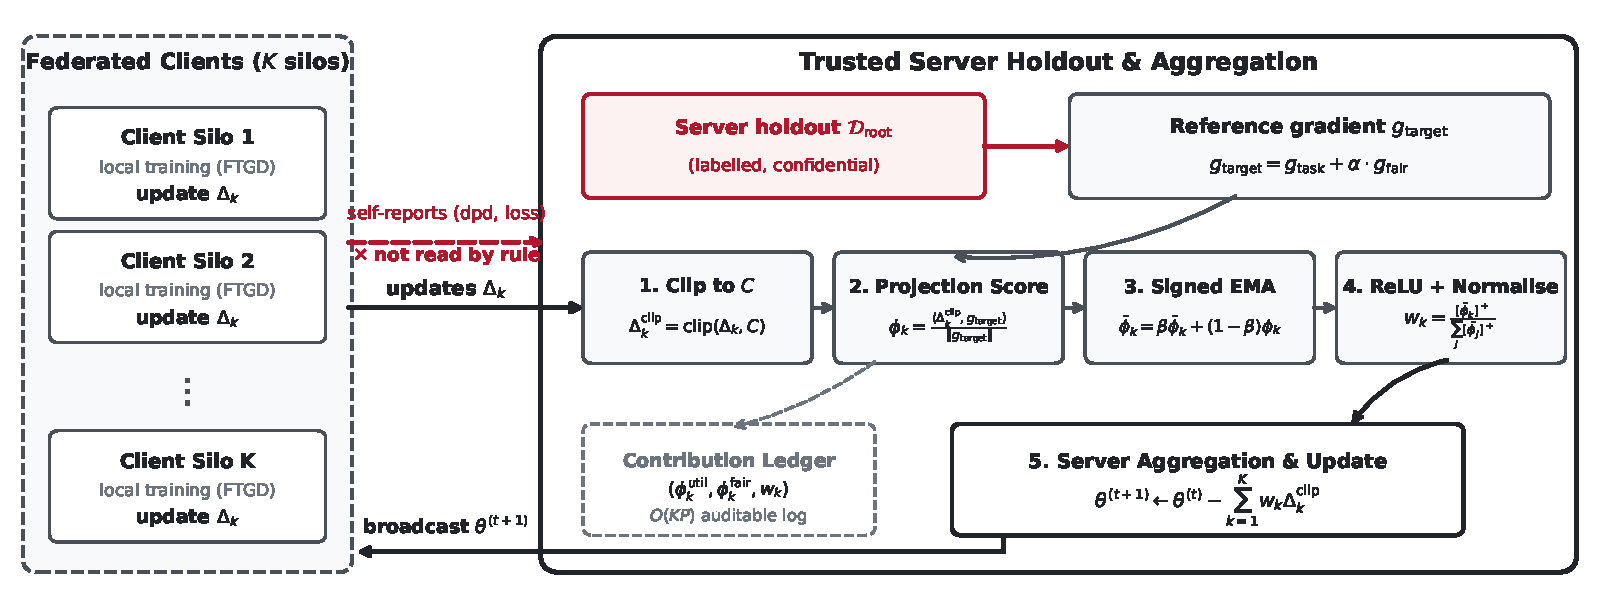
\includegraphics[width=\linewidth]{figures/fig_pipeline.pdf}}{\fbox{\parbox{0.9\linewidth}{\centering Figure in preparation.}}}
\caption{\textbf{FU-Alignment.} Clients send only their updates; the reports that report-reading rules depend on are not read. The server computes a reference gradient on its own holdout graph, clips each update, scores it by its projection onto the reference, smooths the scores over rounds, and averages the clipped updates with weights proportional to the positive part of the smoothed scores. The two parts of each score are logged for audit.}
\label{fig:pipeline}
\end{figure}

\paragraph{Server reference}
Before the clients are formed, the server sets aside up to 200 nodes of the label-stratified validation split, and never more than half of it, as its holdout $\Droot$ (125 nodes on German Credit and 200 on the larger graphs). No client owns these nodes, and no edge connects them to a client subgraph. In round $t$ the server evaluates two gradients on $\Droot$ at the current global model:
\begin{equation}
\label{eq:srv_grads}
\begin{gathered}
\gtask^{\mathrm{srv}} = \nabla_\theta \mathcal{L}_{\mathrm{task}}(\theta^{(t)}; \Droot), \qquad \gfair^{\mathrm{srv}} = \nabla_\theta \mathcal{L}^{\mathrm{srv}}_{\mathrm{fair}}(\theta^{(t)}; \Droot), \\
\mathcal{L}^{\mathrm{srv}}_{\mathrm{fair}} = (\mu_0^{\mathrm{srv}} - \mu_1^{\mathrm{srv}})^2,
\end{gathered}
\end{equation}
where $\mu_a^{\mathrm{srv}}$ is the mean soft prediction for group $a$ on $\Droot$. The squared gap is differentiable at zero, and the server computes it on its own data without noise. The reference combines the two gradients with a fixed weight $\alpha \ge 0$:
\begin{equation}
\label{eq:gtarg_def}
\gtarg^{(t)} = \gtask^{\mathrm{srv}} + \alpha\, \gfair^{\mathrm{srv}}.
\end{equation}
The fairness term tilts the reference towards lower disparity on the holdout. It does not filter clients by itself, and at $\alpha = 0.1$ its measured effect on allocation is negligible (Section~\ref{subsec:rq2_rq3_efficacy}).

\paragraph{Scoring and aggregation}
Each client update $\Delta_k^{(t)} = \theta^{(t)} - \theta_k^{(t)}$ is first clipped to norm $C$,
\begin{equation}
\label{eq:clip_pre_score}
\Delta_k^{\mathrm{clip}(t)} = \Delta_k^{(t)} \cdot \min\left(1, \frac{C}{\norm{\Delta_k^{(t)}}_2}\right),
\end{equation}
and then scored by its projection onto the reference,
\begin{equation}
\label{eq:score_raw}
\varphi_k^{(t)} = \frac{\ip{\Delta_k^{\mathrm{clip}(t)}}{\gtarg^{(t)}}}{\norm{\gtarg^{(t)}}_2}.
\end{equation}
An update that would raise the server's holdout objective, such as a sign-flipped one, receives a negative score. The signed scores are smoothed over rounds,
\begin{equation}
\label{eq:ema_smooth}
\bar{\varphi}_k^{(0)} = \varphi_k^{(0)}, \qquad \bar{\varphi}_k^{(t)} = \beta\, \bar{\varphi}_k^{(t-1)} + (1-\beta)\, \varphi_k^{(t)} \quad (t \ge 1),
\end{equation}
and only then rectified and normalised,
\begin{equation}
\label{eq:weights_simplex}
w_k^{(t)} = \frac{\ReLU(\bar{\varphi}_k^{(t)}) \cdot \mathbb{I}(\norm{\Delta_k^{(t)}} > 0)}{\sum_{j=1}^K \ReLU(\bar{\varphi}_j^{(t)}) \cdot \mathbb{I}(\norm{\Delta_j^{(t)}} > 0)},
\end{equation}
with uniform weights over the clients with a non-zero update if no smoothed score is positive. The global model moves by the weighted clipped updates:
\begin{equation}
\label{eq:model_update}
\theta^{(t+1)} = \theta^{(t)} - \sum_{k=1}^K w_k^{(t)} \Delta_k^{\mathrm{clip}(t)}.
\end{equation}
The canonical FU-Alignment cells use $\alpha = 0.1$, $\beta = 0.9$, and $C = 10$; campaign manifests record any campaign-specific variation.

\paragraph{Design rationale}
Each element answers a weakness identified in Section~\ref{subsec:theory}; Sections~\ref{subsec:rq4_boundary} and~\ref{subsec:rq2_rq3_efficacy} evaluate the resulting rule as a whole.
\begin{enumerate}[leftmargin=*, label=(\roman*)]
    \item \textbf{The reference does not depend on the clients.} Its task and fairness signals are computed on server-held data.
    \item \textbf{The score bounds magnitude and keeps direction.} Clipping before scoring caps what a single update can contribute to its score and to the aggregate (Proposition~\ref{prop:bounded_influence}), while the projection retains its component along the reference. The factorial ablation in Section~\ref{subsec:rq2_rq3_efficacy} shows that replacing clipping by rescaling increases adversarial weight.
    \item \textbf{The score remembers its sign.} Because the signed score is smoothed before it is rectified, a client that turns against the reference loses its weight within a bounded number of rounds (Proposition~\ref{prop:bounded_influence}), and a client that has opposed the reference must point towards it for several rounds before it regains weight.
\end{enumerate}

Table~\ref{tab:rule_comparison} sets these choices against FLTrust and GuardFed, the two server-anchored rules closest to ours.

\begin{table}[t]
\centering
\footnotesize
\caption{\textbf{FU-Alignment against the closest server-anchored rules.} The three rules all score clients against data held by the server; they differ in what the score measures, how update magnitude is handled, and whether scores carry memory. FLTrust and GuardFed as described in~\citep{cao2021fltrust, li2025guardfed}.}
\label{tab:rule_comparison}
\setlength{\tabcolsep}{4pt}
\begin{tabular}{p{0.17\linewidth}p{0.24\linewidth}p{0.26\linewidth}p{0.24\linewidth}}
\toprule
 & \textbf{FLTrust} & \textbf{GuardFed} & \textbf{FU-Alignment} \\
\midrule
Reference & server model update on root data & update of a reference model trained on server and synthetic data with fairness reweighting & task gradient plus $\alpha$ times a fairness gradient on the holdout \\
Client score & ReLU of the cosine with the reference & ReLU of the cosine, times $e^{-\tau_{\mathrm{G}} g_k}$, where $g_k$ is the equal-opportunity gap of the client model & projection of the clipped update onto the reference \\
Update magnitude & every update rescaled to the reference norm & not modified & clipped to norm $C$ \\
Memory & none & none & EMA of the signed score, before rectification \\
Weights & proportional to the score & uniform over clients whose score exceeds $\Gamma_{\mathrm{G}}$ & proportional to the positive part of the smoothed score \\
Server work per round & one update on root data and $K$ cosines & a reference update, $K$ cosines and $K$ model evaluations & two gradients on the holdout and $K$ inner products \\
\bottomrule
\end{tabular}
\end{table}

\begin{proposition}[Bounded influence]
\label{prop:bounded_influence}
Let the weights be given by Eq.~\eqref{eq:weights_simplex}, including the uniform fallback, and the global update by Eq.~\eqref{eq:model_update}.
\begin{enumerate}[leftmargin=*, label=(\roman*)]
    \item Whatever finite updates the clients send, $\norm{\theta^{(t+1)} - \theta^{(t)}}_2 \le C$.
    \item Suppose that client $k$ has $\varphi_k^{(t)} \le -m$ for some $m > 0$ and all $t \ge t_0 \ge 1$. Then $\bar{\varphi}_k^{(t)} \le 0$, and hence $w_k^{(t)} = 0$ whenever the fallback is not used, for all $t \ge t_0 + s - 1$ with
    \begin{equation}
    \label{eq:bounded_rounds}
    s = \left\lceil \frac{\log\left( (C + m)/m \right)}{\log(1/\beta)} \right\rceil .
    \end{equation}
\end{enumerate}
\end{proposition}
\begin{proof}
(i) In both branches the weights are non-negative and sum to one, and $\norm{\Delta_k^{\mathrm{clip}(t)}}_2 \le C$, so $\norm{\sum_k w_k^{(t)} \Delta_k^{\mathrm{clip}(t)}}_2 \le \sum_k w_k^{(t)} \norm{\Delta_k^{\mathrm{clip}(t)}}_2 \le C$.
(ii) By the Cauchy--Schwarz inequality $|\varphi_k^{(t)}| \le \norm{\Delta_k^{\mathrm{clip}(t)}}_2 \le C$ for every $t$, and therefore $\bar{\varphi}_k^{(t)} \le C$, since it is a convex combination of scores. Unrolling Eq.~\eqref{eq:ema_smooth} for $n \ge 1$ rounds from $t_0 - 1$ gives
$\bar{\varphi}_k^{(t_0 - 1 + n)} = \beta^{n} \bar{\varphi}_k^{(t_0-1)} + (1-\beta) \sum_{j=0}^{n-1} \beta^{j} \varphi_k^{(t_0 - 1 + n - j)} \le \beta^{n} C - m (1 - \beta^{n})$,
which is non-positive as soon as $\beta^{n} \le m/(C+m)$, that is, for all $n \ge s$. A non-positive smoothed score has zero rectified value, so the numerator of Eq.~\eqref{eq:weights_simplex} vanishes.
\end{proof}

Part (i) means that no update, however large, can move the global model by more than $C$ in one round. Part (ii) means that a client that persistently opposes the reference loses its weight after at most $s$ rounds. If it opposes the reference in every round from the first one, Eq.~\eqref{eq:ema_smooth} gives $\bar{\varphi}_k^{(t)} \le -m$ in every round by induction, so its weight is zero from the start whenever the fallback is not used; the delay of $s$ rounds applies only to a client that first builds up positive history, and for small $m$ it can exceed the length of our runs. Neither part bounds the weight of an adversary whose update is aligned with the reference; Section~\ref{sec:experiments} measures that case.

\paragraph{Server requirements and cost}
The server needs a holdout of at most $200$ labelled nodes with their sensitive attribute. In each round it evaluates two gradients on the holdout, clips the $K$ updates and computes $K$ inner products, which costs $O(KP)$ in addition to the two gradient evaluations. The clients run standard local training and need to send only their updates.

\begin{algorithm}[t]
\footnotesize
\caption{One round of FU-Alignment}
\label{alg:trustfedgnn}
\begin{algorithmic}[1]
\REQUIRE Global model $\theta^{(t)}$, holdout $\Droot$, smoothed scores $\bar{\varphi}^{(t-1)}$, $\alpha = 0.1$, $\beta = 0.9$, $C = 10$.
\ENSURE $\theta^{(t+1)}$, $\bar{\varphi}^{(t)}$ and the ledger entries of round $t$.
\STATE Compute $\gtask^{\mathrm{srv}}$ and $\gfair^{\mathrm{srv}}$ on $\Droot$ and set $\gtarg^{(t)} \gets \gtask^{\mathrm{srv}} + \alpha \gfair^{\mathrm{srv}}$ \hfill Eqs.~\eqref{eq:srv_grads}--\eqref{eq:gtarg_def}
\STATE Broadcast $\theta^{(t)}$; each client $k$ trains locally (Section~\ref{subsec:client_side}) and returns $\Delta_k^{(t)}$
\FOR{each client $k \in [K]$}
    \STATE $\Delta_k^{\mathrm{clip}(t)} \gets \Delta_k^{(t)} \cdot \min(1, C / \norm{\Delta_k^{(t)}}_2)$ \hfill Eq.~\eqref{eq:clip_pre_score}
    \STATE $\varphi_k^{(t)} \gets \ip{\Delta_k^{\mathrm{clip}(t)}}{\gtarg^{(t)}} / \norm{\gtarg^{(t)}}_2$ \hfill Eq.~\eqref{eq:score_raw}
    \STATE $\bar{\varphi}_k^{(t)} \gets \varphi_k^{(t)}$ if $t = 0$, else $\beta \bar{\varphi}_k^{(t-1)} + (1-\beta) \varphi_k^{(t)}$ \hfill Eq.~\eqref{eq:ema_smooth}
\ENDFOR
\STATE Compute $w^{(t)}$ by Eq.~\eqref{eq:weights_simplex}, with the uniform fallback over clients with $\Delta_k^{(t)} \ne \mathbf{0}$
\STATE $\theta^{(t+1)} \gets \theta^{(t)} - \sum_k w_k^{(t)} \Delta_k^{\mathrm{clip}(t)}$ \hfill Eq.~\eqref{eq:model_update}
\STATE Log $\langle t, k, w_k^{(t)}, \varphi_k^{\mathrm{util}}, \varphi_k^{\mathrm{fair}} \rangle$ for every $k$ \hfill Eq.~\eqref{eq:audit_tuple}
\end{algorithmic}
\end{algorithm}

% =========================================================================
\subsection{Client-Side Training Stack}
\label{subsec:client_side}

To isolate the server-side aggregation mechanism, all methods evaluated in this paper use a common local training stack that adapts the FSER and FTGD ideas from our prior work~\citep{dang2026fedfairgnn}. These fixed client-side components are not claimed as contributions of this study. TrustFedGNN's aggregation path consumes model updates and server-computed reference signals without using client-reported fairness or performance statistics.

The local backbone is a two-layer GAT~\citep{velickovic2017graph} with hidden dimension $64$, batch normalisation, and residual connections, combined with fairness-sensitive edge reweighting (FSER), which initially attenuates inter-group edges by a factor $\gamma_{\mathrm{init}} = 0.5$. Local training adapts fair targeted gradient descent (FTGD). Each client computes a task gradient and the gradient of a fairness loss $\mathcal{L}_{\mathrm{fair}} = |\mu_{k,0} - \mu_{k,1}|$ built from its group means; when report privatisation is enabled, the released means $\tilde{\mu}_{k,a}$ of Eq.~\eqref{eq:scalar_dp} replace them and are computed by a forward pass that does not take $S$ as input:
\begin{equation}
\label{eq:local_grads}
g_{k,\mathrm{task}} = \nabla_\theta \mathcal{L}_{\mathrm{task}}(\theta; \mathcal{G}_k), \qquad g_{k,\mathrm{fair}} = \nabla_\theta \mathcal{L}_{\mathrm{fair}}(\theta; \mathcal{G}_k).
\end{equation}
It removes from the task gradient its component along the fairness gradient,
\begin{equation}
\label{eq:ftgd_proj}
g_k^{\perp} = \begin{cases}
g_{k,\mathrm{task}} - \dfrac{\ip{g_{k,\mathrm{task}}}{g_{k,\mathrm{fair}}}}{\norm{g_{k,\mathrm{fair}}}^2}\, g_{k,\mathrm{fair}}, & \norm{g_{k,\mathrm{fair}}} \ge 10^{-8}, \\
g_{k,\mathrm{task}}, & \text{otherwise},
\end{cases}
\end{equation}
so that $\ip{g_k^{\perp}}{g_{k,\mathrm{fair}}} = 0$, and steps along
\begin{equation}
\label{eq:ftgd_update_step}
u_k = g_k^{\perp} + g_{k,\mathrm{fair}}.
\end{equation}

To run every rule under a common protocol, each client also exports a report containing its training-set size, validation AUC, loss, disparity, and equal opportunity gap; when privatisation is enabled, the reported disparity is the privatised one. FU-Alignment and FLTrust never read this report; CGSV reads only the sample count in a fallback branch, while the report exists for the rules that read it. Privatisation therefore protects a channel that FU-Alignment does not use.

% =========================================================================
\subsection{Contribution Ledger}
\label{subsec:governance}

Because the reference is a sum of two gradients, each score splits exactly into a utility part and a fairness part.

\begin{proposition}[Linear decomposition]
\label{prop:linear_shapley}
For every client and round,
\begin{equation}
\label{eq:linear_decomp}
\varphi_k^{(t)} = \varphi_k^{\mathrm{util}} + \varphi_k^{\mathrm{fair}}, \qquad
\varphi_k^{\mathrm{util}} = \frac{\ip{\Delta_k^{\mathrm{clip}(t)}}{\gtask^{\mathrm{srv}}}}{\norm{\gtarg^{(t)}}_2}, \quad
\varphi_k^{\mathrm{fair}} = \frac{\alpha \ip{\Delta_k^{\mathrm{clip}(t)}}{\gfair^{\mathrm{srv}}}}{\norm{\gtarg^{(t)}}_2},
\end{equation}
and both parts cost $O(KP)$ per round.
\end{proposition}
\begin{proof}
The inner product is linear in its second argument and $\gtarg^{(t)} = \gtask^{\mathrm{srv}} + \alpha \gfair^{\mathrm{srv}}$; dividing by the common normaliser preserves the identity.
\end{proof}

In every round the server appends
\begin{equation}
\label{eq:audit_tuple}
\mathcal{T}_k^{(t)} = \left\langle t, k, w_k^{(t)}, \varphi_k^{\mathrm{util}}, \varphi_k^{\mathrm{fair}} \right\rangle
\end{equation}
to a round log, which records how much of each client's score came from utility and how much from fairness. The implementation stores both parts before the division by $\norm{\gtarg^{(t)}}_2$, which leaves their ratio unchanged. By construction of Eq.~\eqref{eq:weights_simplex}, the weights lie on the probability simplex and a client that sends a zero update receives zero weight. The decomposition is a first-order attribution and does not approximate Shapley values.

\section{Experimental Design and Results}
\label{sec:experiments}

We organize the evaluation around four questions. RQ1 asks whether changing only a client report changes its aggregation weight. RQ2 asks whether FU-Alignment removes that dependency by construction. RQ3 compares FU-Alignment with a faithful root-update FLTrust control under a matched fairness-poisoning protocol and asks which of its components matter. RQ4 tests where the observed behavior persists or fails under different adversarial access schedules and a corrected label protocol. The studies use different federation sizes and horizons (Table~\ref{tab:protocol}), so numbers are compared only within a study.

\subsection{Experimental Design}
\label{subsec:setup}

\paragraph{Datasets}
German Credit (1,000 nodes, 21,742 edges, sensitive attribute gender) and Bail Recidivism (18,876 nodes, 311,870 edges, race) follow the NIFTY preprocessing~\citep{agarwal2021towards}; Pokec-z (67,796 nodes, 617,958 edges, region) follows FairGNN~\citep{dai2021say,takac2012data}. On Pokec-z we evaluate only the 10,262 nodes with an observed label (15.1\%) rather than treating missing labels as negatives. Before partitioning, the server removes its holdout $\Droot$ from the label-stratified validation split: $\min(200, |\mathcal{V}_{\mathrm{val}}|/2)$ nodes, which is 125 nodes on German and 200 on Bail and Pokec-z. The remaining nodes are split across $K$ clients by a Dirichlet label skew with concentration 0.3; edges between clients and edges to the holdout are dropped.

\paragraph{Training}
Clients train full-batch for three local epochs per round with AdamW (learning rate 0.01, weight decay $10^{-5}$). Except in the two report audits, every method uses the same client stack (Section~\ref{subsec:client_side}): a two-layer GAT with FSER and FTGD. Because the audits test only the aggregation interface, they hold a two-layer GCN client trained with FTGD fixed across all rules; the fixed-update audit uses a 100-node holdout and the end-to-end audit the default holdout above. Report privatisation is enabled only in the Pokec-z control ($\epsilon = 8$) and in the report-privacy diagnostic; elsewhere FTGD uses exact group means. FU-Alignment uses $\alpha = 0.1$, $\beta = 0.9$, and $C = 10$. The factorial cells and the adaptive-access study use a cosine variant of the score, $\cos(\Delta_k^{\mathrm{clip}}, \gtarg)/\norm{\gtarg}_2$, in place of the projection of Eq.~\eqref{eq:score_raw}; in the controlled study its adversarial weight is close to that of the projection score (0.074 versus 0.063 on German, SR+C cell of Table~\ref{tab:c23_factorial}). Because this score is not bounded by $C$, Proposition~\ref{prop:bounded_influence}(ii) does not apply to it directly.

\paragraph{Attacks}
In \emph{fairness poisoning}, each adversarial client trains on its own data to minimise $\mathcal{L}_{\mathrm{BCE}} - 10\,\widehat{\dpd}_{\mathrm{soft}}$, that is, to increase disparity while keeping some predictive signal, and reports $\widehat{\dpd} = 0$ with near-perfect utility. The fixed-update audit uses the same update but switches only the report between honest and falsified values. The adaptive-access study varies when and how the adversary acts over 40 rounds:
\begin{itemize}[leftmargin=*]
    \item \textbf{Sustained poisoning:} honest in rounds 0--9, fairness poisoning from round 10 onward.
    \item \textbf{Intermittent poisoning:} honest in rounds 0--9, then alternating five poisoning rounds and five honest rounds, so that honest phases can rebuild the adversary's score history.
    \item \textbf{Reference evasion:} from round 1 the adversaries send one crafted update, initialised at the adversary's honest update and optimised for 50 steps to align with the previous global step (a public surrogate of the server reference) while opposing the adversary's own fairness gradient, with a penalty on any norm above five times that of the honest update. The adversary never sees $\Droot$.
\end{itemize}

\paragraph{Comparators and metrics}
The audit covers six report-dependent rules (FairFed, $q$-FFL-eq, $F^2$GNN, FedGraph-Fair, PoPETs-FairFed, and BFWA) and four rules that do not read the audited report (CGSV, FLTrust, root-update FLTrust, and FU-Alignment). Root-update FLTrust computes its reference update on the same server holdout as FU-Alignment and is the faithful control in every later study. The adaptive-access study adds FedAvg and a GuardFed-style comparator whose two hyperparameters were selected on separate tuning seeds at $K=5$ with one adversary and then frozen and reused at $K=10$ (Section~S1 of ESM~1); we label it as an adaptation because the holdout and implementation details differ from the original~\citep{li2025guardfed}. We report AUC, DPD, and EOD on the test split; DPD and EOD use hard predictions at a 0.5 threshold. The adversarial weight $w_{\rm adv}$ is the total aggregation weight of the adversarial clients, averaged over rounds (in the adaptive-access study, over the rounds in which the adversaries poison). The processed influence $I_{\rm adv} = \|\sum_{i \in \mathcal{A}} w_i \tilde{\Delta}_i\|_2$, also averaged over rounds, measures how far the adversarial contributions move the model after each rule's own clipping or rescaling $\tilde{\Delta}_i$.

\paragraph{Statistics}
Seeds are paired within each study: the partition, holdout, and initialisation are identical across rules for a given seed. We report paired mean differences with 95\% bootstrap confidence intervals and two-sided Wilcoxon signed-rank tests, with Holm correction across the eight dataset--metric contrasts against root-update FLTrust and across those of the $\alpha = 0$ comparison; contrasts against FedAvg are reported unadjusted. The Pokec-z control tests non-inferiority against a margin of 0.01 AUC, fixed before the run, using the one-sided 95\% bootstrap lower bound.

\begin{table*}[t]
\centering
\scriptsize
\caption{\textbf{Evaluation protocol.} Each study answers one research question with its own federation size and number of rounds $R$; results are compared only within a study. $K$ is the number of clients and $f$ the number of adversaries. The last column gives the identifier of the corresponding artifact in the code repository.}
\label{tab:protocol}
\setlength{\tabcolsep}{3pt}
\resizebox{\textwidth}{!}{%
\begin{tabular}{llllrrll}
\toprule
\textbf{Study} & \textbf{RQ} & \textbf{Data} & \textbf{$K$/$f$} & \textbf{$R$} & \textbf{Seeds} & \textbf{Rules} & \textbf{Artifact} \\
\midrule
Fixed-update audit & 1, 2 & German & 5 / 1 & 20 & 30 & 10 rules (Table~\ref{tab:c20_report_audit}) & C20r \\
End-to-end audit & 1 & German, Bail & 5 / 1 & 20 & 30 & root-FLTrust & C20b/c \\
Controlled fairness poisoning & 3 & German, Bail & 5 / 1 & 20 & 30 & FU-Alignment, root-FLTrust, FedAvg; factorial; $\alpha = 0$ & C23, C23b, C26 \\
Adaptive access & 4 & German, Bail & 10 / 2 & 40 & 10 & FedAvg, root-FLTrust, FU-Alignment, GuardFed-style & C24 \\
Known-label control & 4 & Pokec-z & 10 / 0 & 50 & 10 & FedAvg, FU-Alignment & C25 \\
\bottomrule
\end{tabular}}
\end{table*}

\subsection{RQ1: Does Falsified Telemetry Change Trust Allocation?}
\label{subsec:rq1_audit}

The fixed-update audit replays the same client updates, server state and server reference twice and changes only the adversary's report. Report-dependent rules receive the lie that best serves the adversary under each rule; the report-free rules receive a report in which every field except the sample count is falsified. This design tests the aggregation interface rather than the success of a jointly trained attack.

%% generated by experiments/campaigns/make_tables.py -- do not edit by hand
%% source: results/campaigns/C20r_fixed_state_replay.json (commit 671ca8cd)
\begin{table}[t]
\centering
\footnotesize
\caption{\textbf{Fixed-update intervention isolates sensitivity to a falsified client report.} In both arms the client updates, server state and server reference are identical; only the adversary's report changes. Report-dependent rules receive their best-response lie; the report-free rules below the line receive a report in which every field except the sample count is falsified. Means over 30 seeds and 20 rounds on German Credit. The final column counts seeds with a nonzero change.}
\label{tab:c20_report_audit}
\setlength{\tabcolsep}{5pt}
\begin{tabular}{lrrrr}
\toprule
\textbf{Aggregation rule} & $w_{\rm adv}^{\rm honest}$ & $w_{\rm adv}^{\rm false}$ & $\Delta w_{\rm adv}$ & \textbf{Nonzero} \\
\midrule
FairFed & 0.0703 & 0.2387 & 0.1684 & 30/30 \\
$q$-FFL-eq & 0.1999 & 0.5050 & 0.3051 & 30/30 \\
$F^2$GNN & 0.0718 & 0.9802 & 0.9084 & 30/30 \\
FedGraph-Fair & 0.2210 & 0.2605 & 0.0395 & 26/30 \\
PoPETs-FairFed & 0.1773 & 0.1854 & 0.0080 & 30/30 \\
BFWA & 0.0707 & 0.7204 & 0.6497 & 25/30 \\
\midrule
CGSV & 0.1918 & 0.1918 & 0.0000 & 0/30 \\
FLTrust & 0.3209 & 0.3209 & 0.0000 & 0/30 \\
root-update FLTrust & 0.1624 & 0.1624 & 0.0000 & 0/30 \\
FU-Alignment & 0.1079 & 0.1079 & 0.0000 & 0/30 \\
\bottomrule
\end{tabular}
\end{table}


Every audited report-dependent rule responds in at least 25 of 30 seeds, whereas CGSV, both FLTrust variants, and FU-Alignment do not respond in any seed: their weights and their aggregate are bit-identical under the honest and the falsified report (Table~\ref{tab:c20_report_audit}). The magnitude varies sharply across rules; the mean adversarial-weight change is 0.908 for $F^2$GNN, 0.650 for BFWA, and 0.305 for $q$-FFL-eq. These values measure an input dependency of the evaluated implementations.

An end-to-end audit, in which the adversary trains jointly with the federation and falsifies its report in every round, confirms the invariance for root-update FLTrust: its mean adversarial weight is the same with and without the lie (0.143 on German, 0.129 on Bail). A separate diagnostic of privatised reports, confined to the scalar report channel and BFWA's decision, is in Section~S2 of ESM~1.

\subsection{RQ2--RQ3: Report Independence and Controlled Efficacy}
\label{subsec:rq2_rq3_efficacy}

FU-Alignment never reads the audited client telemetry, so the fixed-update audit verifies report independence for the implemented aggregation path. The controlled study then asks a different question: how does that path behave under matched fairness poisoning when compared with root-update FLTrust?

%% generated by experiments/campaigns/make_tables.py -- do not edit by hand
%% source: results/campaigns/C23_mechanism_factorial.json (commit c9fa8248)
%% source: results/campaigns/analysis/discover_ai.json (commit derived)
\begin{table*}[t]
\centering
\scriptsize
\caption{\textbf{Controlled fairness-poisoning comparison.} Panel A gives means over 30 paired seeds ($K=5$, one adversary). Panel B gives FU-Alignment minus comparator with paired 95\% bootstrap confidence intervals. Against root-update FLTrust, Holm correction across the eight dataset--metric tests retains $w_{\rm adv}$ and AUC on both datasets and EOD on German; neither DPD contrast nor Bail EOD is significant. Against FedAvg, $w_{\rm adv}$, DPD and EOD decrease on both datasets at unadjusted $p<0.05$, while Bail AUC decreases. DPD and EOD use a 0.5 decision threshold.}
\label{tab:c23_controlled}
\setlength{\tabcolsep}{4pt}
\textbf{A. Endpoint means}\\[2pt]
\begin{tabular}{llrrrr}
\toprule
\textbf{Dataset} & \textbf{Rule} & $w_{\rm adv}$ & \textbf{AUC} & \textbf{DPD} & \textbf{EOD} \\
\midrule
German & FedAvg & 0.1649 & 0.6260 & 0.1550 & 0.1626 \\
German & root-update FLTrust & 0.1892 & 0.6205 & 0.1165 & 0.1361 \\
German & FU-Alignment & 0.0630 & 0.6414 & 0.0720 & 0.0688 \\
Bail & FedAvg & 0.1939 & 0.7381 & 0.0366 & 0.0546 \\
Bail & root-update FLTrust & 0.1959 & 0.6990 & 0.0265 & 0.0495 \\
Bail & FU-Alignment & 0.0451 & 0.7234 & 0.0197 & 0.0361 \\
\bottomrule
\end{tabular}\\[5pt]
\textbf{B. Paired difference: FU-Alignment minus comparator}\\[2pt]
\resizebox{\textwidth}{!}{%
\begin{tabular}{llrrrr}
\toprule
\textbf{Dataset} & \textbf{Comparator} & $\Delta w_{\rm adv}$ [95\% CI] & $\Delta$ AUC [95\% CI] & $\Delta$ DPD [95\% CI] & $\Delta$ EOD [95\% CI] \\
\midrule
German & root-FLTrust & $-0.126$ [$-0.149, -0.103$] & $+0.021$ [$+0.006, +0.036$] & $-0.045$ [$-0.084, -0.010$] & $-0.067$ [$-0.114, -0.025$] \\
German & FedAvg & $-0.102$ [$-0.164, -0.047$] & $+0.015$ [$-0.001, +0.034$] & $-0.083$ [$-0.146, -0.027$] & $-0.094$ [$-0.170, -0.029$] \\
Bail & root-FLTrust & $-0.151$ [$-0.185, -0.114$] & $+0.024$ [$+0.005, +0.043$] & $-0.007$ [$-0.019, +0.004$] & $-0.013$ [$-0.027, +0.000$] \\
Bail & FedAvg & $-0.149$ [$-0.201, -0.103$] & $-0.015$ [$-0.027, -0.002$] & $-0.017$ [$-0.033, -0.004$] & $-0.018$ [$-0.033, -0.005$] \\
\bottomrule
\end{tabular}}
\end{table*}


FU-Alignment assigns lower mean adversarial weight than root-update FLTrust on both datasets: 0.0630 versus 0.1892 on German (lower in 29 of 30 paired seeds) and 0.0451 versus 0.1959 on Bail (27 of 30) (Table~\ref{tab:c23_controlled}). It also has higher AUC on both datasets (+0.021 and +0.024). With Holm correction across the eight dataset--metric contrasts, both allocation reductions, both AUC gains, and the German EOD reduction remain significant; the DPD contrasts and the Bail EOD contrast do not. Against FedAvg in the same runs, FU-Alignment lowers adversarial weight, DPD, and EOD on both datasets, at the cost of 0.015 AUC on Bail. A logged replay reproduces these runs bit for bit and records per-round weights, scores, and $I_{\rm adv}$; FU-Alignment's mean processed influence is 0.401 against 1.172 for root-update FLTrust on German (lower in 29 of 30 seeds) and 0.319 against 1.275 on Bail (26 of 30).

%% generated by experiments/campaigns/make_tables.py -- do not edit by hand
%% source: results/campaigns/analysis/discover_ai.json (commit derived)
\begin{table*}[t]
\centering
\scriptsize
\caption{\textbf{Factorial mechanism ablation under fairness poisoning.} Mean adversarial weight for smooth--rectify (SR) or rectify--smooth (RS), combined with clipping (C) or rescaling (R), over 30 paired seeds. All four cells score updates by $\cos(\Delta_k, g)/\lVert g \rVert$. Positive factorial effects mean that rectify-first or rescaling increases adversarial allocation. Brackets are paired 95\% bootstrap confidence intervals.}
\label{tab:c23_factorial}
\resizebox{\textwidth}{!}{%
\begin{tabular}{lrrrrrr}
\toprule
\textbf{Dataset} & \textbf{SR+C} & \textbf{SR+R} & \textbf{RS+C} & \textbf{RS+R} & \textbf{Order effect} & \textbf{Magnitude effect} \\
\midrule
German & 0.074 & 0.157 & 0.115 & 0.186 & +0.035 [+0.022,+0.049] & +0.077 [+0.053,+0.099] \\
Bail & 0.046 & 0.080 & 0.078 & 0.097 & +0.024 [+0.016,+0.034] & +0.027 [+0.018,+0.036] \\
\bottomrule
\end{tabular}}
\end{table*}


\paragraph{Which components produce the reduction}
Both methods use server data, so the empirical question is which of FU-Alignment's departures from FLTrust matter. A $2 \times 2$ factorial within the same protocol, using the cosine score in all four cells, varies the order of smoothing and rectification and the treatment of update magnitude (Table~\ref{tab:c23_factorial}). Rectifying before smoothing raises adversarial weight by 0.035 on German and 0.024 on Bail, and rescaling updates to a common norm instead of clipping raises it by 0.077 and 0.027; all four paired confidence intervals exclude zero. Signed smoothing and clipping therefore both contribute. A paired run with the fairness term removed ($\alpha = 0$, all else equal) isolates the reference itself: at $\alpha = 0.1$ the fairness term lowers German adversarial weight by only 0.003 (Holm-adjusted $p = 0.011$) and changes no other endpoint detectably on either dataset. The reduction relative to root-update FLTrust is therefore attributable to how updates are processed and scored over time, not to the fairness direction at this weight.

\subsection{RQ4: Adaptive-Access and Label-Protocol Boundaries}
\label{subsec:rq4_boundary}

The adaptive-access study contains 320 runs over German and Bail, four methods, three attack schedules plus benign controls, and 10 paired seeds. Table~\ref{tab:c24_boundary} reports weight and influence over the rounds in which the adversaries poison; Section~S3 of ESM~1 gives all-round means.

Reference evasion, the attack with the most knowledge of the server rule, is the most damaging one for FedAvg: its AUC falls to 0.590 on both datasets, against 0.661 and 0.749 in its benign runs. FU-Alignment gives the adversaries the lowest weight and influence of the four methods on both datasets (0.034 and 0.266 on German, 0.033 and 0.233 on Bail; root-update FLTrust 0.169 and 1.054, and 0.137 and 0.898) and keeps the highest attacked AUC (0.641 on German, 0.709 on Bail). On Bail, FU-Alignment also has the lowest processed influence under sustained and intermittent poisoning; under intermittent poisoning the GuardFed-style adaptation assigns slightly less weight (0.119 versus 0.128) but more influence (1.543 versus 0.660). On German, the GuardFed-style adaptation has the lowest weight and influence under both poisoning schedules.

The boundary is intermittent poisoning on German. There FU-Alignment gives the adversaries more weight and influence (0.210 and 1.237) than FedAvg (0.202 and 1.167) and root-update FLTrust (0.197 and 1.122), whereas under sustained poisoning its weight on the same dataset is 0.126. Each honest phase lets the adversaries rebuild a positive smoothed score that they then spend while poisoning; temporal memory, which removes a persistent opponent, can preserve the influence of one that alternates. The adaptive-access study therefore maps where the advantage holds and where it does not.

%% generated by experiments/campaigns/make_tables.py -- do not edit by hand
%% source: results/campaigns/C24_adaptive_access.json (commit cf844221)
%% source: results/campaigns/C24r_s3_fedavg.json (commit c6a986c4)
%% source: results/campaigns/analysis/discover_ai.json (commit derived)
\begin{table*}[t]
\centering
\scriptsize
\caption{\textbf{Adaptive-access boundary map.} $K=10$ clients, two adversaries, 40 rounds, means over 10 paired seeds. $w_{\rm adv}$ and $I_{\rm adv}$ are averaged over the rounds in which the adversaries poison (from round 10 under sustained poisoning, alternate five-round blocks under intermittent poisoning, every round after the first under reference evasion); AUC, DPD and EOD are final endpoints. On Bail, FU-Alignment has the lowest processed influence under sustained and intermittent poisoning, and under reference evasion it gives the adversaries the lowest weight and influence of the four methods and keeps the highest AUC on both datasets. Intermittent poisoning on German is the boundary: FU-Alignment gives the adversaries more weight and influence than FedAvg and root-FLTrust. All-round means are in the Supplementary Information (ESM 1).}
\label{tab:c24_boundary}
\setlength{\tabcolsep}{4pt}
\begin{tabular}{lllrrrrr}
\toprule
\textbf{Dataset} & \textbf{Attack} & \textbf{Rule} & $w_{\rm adv}$ & $I_{\rm adv}$ & \textbf{AUC} & \textbf{DPD} & \textbf{EOD} \\
\midrule
German & sustained & FedAvg & 0.202 & 1.163 & 0.646 & 0.146 & 0.148 \\
German & sustained & root-FLTrust & 0.196 & 1.122 & 0.652 & 0.155 & 0.106 \\
German & sustained & FU-Alignment & 0.126 & 0.749 & 0.641 & 0.080 & 0.088 \\
German & sustained & GuardFed-style & 0.009 & 0.054 & 0.661 & 0.097 & 0.080 \\
\addlinespace[2pt]
German & intermittent & FedAvg & 0.202 & 1.167 & 0.660 & 0.066 & 0.060 \\
German & intermittent & root-FLTrust & 0.197 & 1.122 & 0.664 & 0.046 & 0.063 \\
German & intermittent & FU-Alignment & 0.210 & 1.237 & 0.650 & 0.058 & 0.078 \\
German & intermittent & GuardFed-style & 0.022 & 0.146 & 0.653 & 0.066 & 0.062 \\
\addlinespace[2pt]
German & reference evasion & FedAvg & 0.202 & 3.272 & 0.590 & 0.219 & 0.232 \\
German & reference evasion & root-FLTrust & 0.169 & 1.054 & 0.624 & 0.167 & 0.187 \\
German & reference evasion & FU-Alignment & 0.034 & 0.266 & 0.641 & 0.060 & 0.077 \\
German & reference evasion & GuardFed-style & 0.049 & 0.656 & 0.629 & 0.073 & 0.064 \\
\addlinespace[2pt]
Bail & sustained & FedAvg & 0.191 & 1.549 & 0.738 & 0.023 & 0.026 \\
Bail & sustained & root-FLTrust & 0.173 & 1.114 & 0.718 & 0.016 & 0.034 \\
Bail & sustained & FU-Alignment & 0.093 & 0.491 & 0.716 & 0.008 & 0.028 \\
Bail & sustained & GuardFed-style & 0.129 & 1.708 & 0.714 & 0.010 & 0.031 \\
\addlinespace[2pt]
Bail & intermittent & FedAvg & 0.191 & 1.745 & 0.749 & 0.015 & 0.024 \\
Bail & intermittent & root-FLTrust & 0.172 & 1.098 & 0.722 & 0.014 & 0.026 \\
Bail & intermittent & FU-Alignment & 0.128 & 0.660 & 0.719 & 0.009 & 0.025 \\
Bail & intermittent & GuardFed-style & 0.119 & 1.543 & 0.724 & 0.012 & 0.028 \\
\addlinespace[2pt]
Bail & reference evasion & FedAvg & 0.191 & 60.738 & 0.590 & 0.064 & 0.071 \\
Bail & reference evasion & root-FLTrust & 0.137 & 0.898 & 0.642 & 0.045 & 0.061 \\
Bail & reference evasion & FU-Alignment & 0.033 & 0.233 & 0.709 & 0.015 & 0.036 \\
Bail & reference evasion & GuardFed-style & 0.048 & 2.762 & 0.665 & 0.016 & 0.031 \\
\bottomrule
\end{tabular}
\end{table*}


%% generated by experiments/campaigns/make_tables.py -- do not edit by hand
%% source: results/campaigns/C25b_control_pokecz_known.json (commit c696a4f0)
\begin{table}[t]
\centering
\footnotesize
\caption{\textbf{Pokec-z known-label control supports AUC non-inferiority, not fairness superiority.} Mean $\pm$ sample SD over 10 paired seeds. FU-Alignment minus FedAvg: AUC $+0.002409$ (Wilcoxon $p=0.375$), DPD $+0.003431$ ($p=0.922$), and EOD $+0.009312$ ($p=0.084$). The prespecified AUC non-inferiority margin is 0.01; the one-sided 95\% bootstrap lower bound is $-0.002060$.}
\label{tab:c25_known_labels}
\setlength{\tabcolsep}{5pt}
\begin{tabular}{lrrr}
\toprule
\textbf{Rule} & \textbf{AUC} & \textbf{DPD} & \textbf{EOD} \\
\midrule
FedAvg & 0.7421 $\pm$ 0.0079 & 0.0286 $\pm$ 0.0214 & 0.0245 $\pm$ 0.0203 \\
FU-Alignment & 0.7445 $\pm$ 0.0104 & 0.0321 $\pm$ 0.0257 & 0.0338 $\pm$ 0.0194 \\
\bottomrule
\end{tabular}
\end{table}


The known-label control tests benign utility under the corrected Pokec-z known-label protocol. FU-Alignment's paired AUC difference from FedAvg is $+0.002409$; the one-sided 95\% bootstrap lower bound is $-0.002060$, above the prespecified $-0.01$ margin. FU-Alignment therefore preserves predictive utility on Pokec-z; its DPD and EOD differences from FedAvg are not significant (Table~\ref{tab:c25_known_labels}).

\section{Discussion}
\label{sec:discussion}

\paragraph{What report independence buys}
The audit separates two questions that are usually asked together. Whether a rule can be moved by what a client says about itself is a property of the aggregation interface, and the fixed-update intervention answers it without training noise. Whether a rule resists what a client sends is a property of the training dynamics, and it depends on the attack. FU-Alignment settles the first question by construction and, in the controlled study, also lowers the weight and processed influence of a fairness-poisoning client relative to root-update FLTrust. The ablation locates that advantage in how updates are processed: clipping before scoring and smoothing the signed score before rectification. Server anchoring alone, which FU-Alignment shares with FLTrust, does not produce it.

\paragraph{Deployment}
The rule needs a small labelled holdout with sensitive attributes at the server. In a cross-silo consortium of lenders or public agencies, such a set can be an audit sample curated by the consortium or held by a supervisor, and it can be kept in a trusted execution environment so that clients never see it. The server's extra work per round is two gradient evaluations on the holdout and one inner product per client, and every round leaves a ledger entry that splits each client's score into utility and fairness parts. An auditor can therefore check after the fact why a client received its weight without access to any client's data. Two properties of the holdout shape what the reference can see. It is carved out before the clients are formed and keeps only the edges among its own nodes, so it is much sparser than the client graphs; on Bail most holdout nodes have no edge at all. The reference gradients are therefore driven mainly by node features, and the server never needs the clients' graph structure. The holdout is also drawn from the same validation distribution as the evaluation split, the premise that FLTrust makes for its root dataset.

\paragraph{Limitations}
Report independence closes one input channel; it does not provide general Byzantine robustness. An adversary whose update aligns with the server reference keeps influence, and an adversary that alternates honest and poisoning phases can exploit the memory of the smoothed score, as intermittent poisoning on German shows. The rule assumes that the holdout is clean, confidential and representative of the federation; a holdout drawn from a shifted population, server compromise and Sybil participation are not tested here. Anchoring to a 200-node holdout has a benign cost on Bail, where FU-Alignment's clean AUC is below FedAvg's, a cost shared by root-update FLTrust. The fairness term of the reference has no detectable effect at the weight used here, so the study does not show that the fairness direction itself improves allocation or fairness; whether a larger weight trades utility for fairness is untested. The privacy analysis covers only the released report channel under a Gaussian approximation and gives no guarantee for model updates. Finally, the three graphs have binary sensitive attributes; intersectional groups, other graph domains and larger federations remain to be studied.

\section{Conclusion}
\label{sec:conclusion}

Aggregation rules that weight clients by what they report about themselves can be steered through those reports. A fixed-update audit makes this measurable: with updates and server state held fixed, every report-dependent rule tested shifts weight towards a client that falsifies its report, while rules that read no report produce identical aggregates.

FU-Alignment removes this channel by scoring clipped updates against a reference gradient that the server computes on its own holdout. Under controlled fairness poisoning it gives the adversary less weight and less processed influence than root-update FLTrust on both datasets, with higher AUC, and a factorial ablation traces the advantage to clipping before scoring and to smoothing the signed score before rectification. Under reference evasion it gives the adversaries the lowest weight and influence of the four rules compared and keeps the highest AUC, and on Pokec-z it preserves the predictive utility of FedAvg. Every round leaves a ledger that splits each client's score into utility and fairness parts, so allocation decisions can be audited after the fact.

The adaptive-access study and Section~\ref{sec:discussion} delimit where these results hold. Natural next steps are holdouts drawn from shifted populations, attackers that alternate phases against the score memory, and federations with more clients and intersectional sensitive groups.


%% =========================================================================
%% BACKMATTER & DECLARATIONS (SPRINGER NATURE STANDARD)
%% =========================================================================

\backmatter

\bmhead{Supplementary information}
The online version contains Supplementary Information (ESM~1): the report-channel privacy analysis with proofs, the complete adaptive-access grid averaged over all rounds, the GuardFed-style tuning protocol, and a supporting stealth-poisoning sweep.

\section*{Declarations}

\bmhead{Funding}
No external funding was received for conducting this study.

\bmhead{Competing interests}
The authors declare that they have no competing financial or non-financial interests that are directly or indirectly related to the work submitted for publication.

\bmhead{Ethics approval}
Not applicable. This study does not involve human participants or live vertebrate animals. All datasets analyzed are publicly available standard machine learning benchmarks.

\bmhead{Consent to participate}
Not applicable.

\bmhead{Consent for publication}
Not applicable.

\bmhead{Data availability}
All datasets analysed in this study are public. German Credit and Bail Recidivism were obtained from the NIFTY benchmark release~\citep{agarwal2021towards} (\url{https://github.com/chirag126/nifty}); Pokec-z was obtained from the FairGNN release~\citep{dai2021say} (\url{https://github.com/EnyanDai/FairGNN}), derived from the Pokec social network~\citep{takac2012data}. Preprocessing, the server-holdout split, and the client partitions are generated by scripts in the code repository from fixed seeds.

\bmhead{Code availability}
The TrustFedGNN source code, experiment runners, per-seed result artifacts, and the verifier that checks them are available at \codeurl. Each result in this article is identified by its artifact ID (Table~\ref{tab:protocol}).

\bmhead{Author contributions}
N.-S.-A. Nguyen: Conceptualization, Methodology, Software, Formal analysis, Investigation, Writing -- original draft. Q.-V. Dang: Supervision, Validation, Writing -- review \& editing. T.-N. Huynh: Supervision, Validation, Writing -- review \& editing. All authors read and approved the final manuscript.

%% =========================================================================
%% BIBLIOGRAPHY
%% =========================================================================
\bibliography{ref}

\end{document}
